\title{N-Graph Notes}
\author{
  Gerrett Diamond\\
}
\date{\today}

\documentclass[12pt]{article}
\usepackage{amsmath}
\usepackage{hyperref}
\usepackage{graphicx}
\begin{document}
\maketitle

\section{Overview} \label{overview}
EnGPar interfaces to the (hyper)graph, geometric, and diffusive dynamic
partitioning procedures through the N-Graph abstraction.

Towards supporting the effective execution of a combination of (hyper)graph,
geometric and diffusive partitioning methods on both graph and mesh data the
N-graph is defined as $G^n(V,E_0,E_1,...,E_{n-1})$ where:
\begin{itemize}
  \item $V$ atomic units $u_i$ of the domain $\omega$ which uniquely exist on one
    part such that $\omega = \bigcup_{\forall_i}u_i$, and 
  \item $E_i$ relations $e_i(u,v)$ of type $i$ between vertices $u$ and $v$
    where $u,v \in V$.
\end{itemize}
Optionally, vertices and edges may be assigned associated weights $w$.  
Vertices may also have a spatial relation in the form of a coordinate vector $c$.
Coordinates define a spatial relation but don't necessarily have to be of $d$
dimensions for a $d$-dimension domain.

\subsection{Hypergraph edges vs Graph edges}
For applications that have data structures that use second adjacencies as edges such as unstructured meshes, converting these second adjacencies into graph edges creates a spider effect for each second adjacency. This leads to a large amount of edges being created and thus is a memory issue. One solution to this problem is to define the edges as hyperedges instead where instead of vertices being connected directly to edges, they are all grouped into a single hyperedge. As a result for these second adjacencies for $m$ graph vertices incident to the second adjacency there will be $2m$ edges created across the second adjacency rather than $m!$ regular graph edges. Therefore we use hyperedges for the relations defined by the N-Graph since traditional graph edges can be defined where hyperedges just act like a regular edge at a cost of an additional $|E|$ memory. A future optimization planned is to add a flag that controls whether to be using hyperedges or not as a way to avoid this extra memory in the case of using traditional graph edges only.

\section{Data Structures}
%Describe the CSR format
The N-Graph data storage is implemented using the commonly used Compressed Sparse
Row (CSR) format to represent the adjacent matrix of the graph. For this structure
there are two arrays. The first is of size $|E|$ and stores the vertex id
at the end of an edge which we will refer to as the edge\_list. The second
which we will refer to as edge\_offsets is of size $|V|+1$ and stores the
offsets into the first array for each vertex. For example see Figure
\ref{fig:simple_graph}. The arrays would look like the following: \\

%TODO: center the figure
\begin{figure}[!h]
  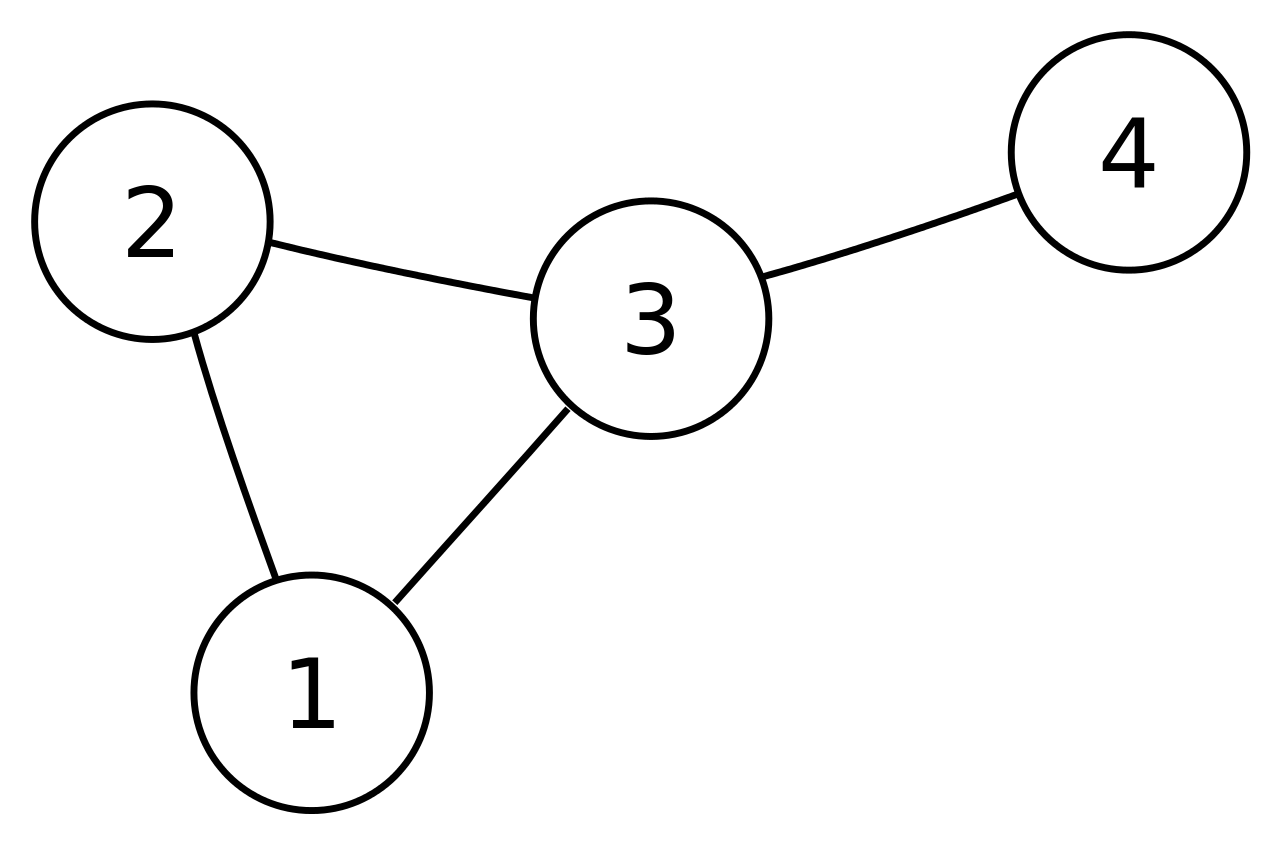
\includegraphics[width=3in]{graph.png}
  \caption{\label{fig:simple_graph}
  }
\end{figure}

\noindent edge\_offset:
\[ \left[ \begin{matrix} 0 & 2 & 4 & 7 & 8\end{matrix} \right] \]
edge\_list:
\[ \left[ \begin{matrix} 2 & 3 & 1 & 3 & 1 & 2 & 4 & 3 \end{matrix} \right] \]

\noindent This structure provides $O(1)$ access to the degree and edges off any
vertex by using the id of the vertex as the index of the edge\_offset array.
The value of the edge\_offset array at that index is the starting index in
the edge\_list for the edge of that vertex. The degree is simply the
difference between the values in the edge\_offset at the following index and
current index. For example vertex three in Figure \ref{fig:simple_graph} has
degree edge\_offset[4]$\ -\ $edge\_offset[3]$\ = 7 - 4 = 3$ and the edges are
found starting at edge\_list[4] which are 1, 2, and 4. To get a full
understanding of how the CSR format is used in the context of the N-Graph
we first describe the data structures in the context of a serial N-Graph
and then in the following section describe the differences when moving to
the distributed N-Graph.

\subsection{Serial Data Structures}
Since the N-Graph utilizes hyperedges, the typical CSR format is altered
to include edge ids as a part of the structures. Thus the N-Graph CSR format
requires four arrays:
\begin{flalign*}
\text{edge\_offset :} & \text{ An array of size } |V|+1 \text{ that stores
offsets into the edge\_list} & \\
\text{edge\_list :} & \text{ An array of size } |P| \text{ that stores hyperedge
ids that the vertex connects to.} \\
\text{pin\_offset :} & \text{ An array of size } |E|+1 \text{ that stores
offsets into the pin\_list}. \\
\text{pin\_list :} & \text{ An array of size } |P| \text{ that stores vertex
ids that the edge connects to.} \\
\end{flalign*}

Each of the offset arrays and the lists operate the same way that they do in
the traditional CSR format providing $O(1)$ access to the degree and edges/pins
of any vertex or hyperedge given the index. It is also important to note that
each of these four arrays exist for each edge type used in the N-Graph. So for
the case of constructing the N-graph from a mesh where the graph vertices
represent mesh elements and there is an edge type for both the mesh vertices
and mesh faces, there would be a total of eight arrays: Four for the adjacency
between the mesh elements and mesh vertices and four for the mesh element and
face adjacency. Along with the four adjacency arrays there are additional arrays
for weights and coordinates that are optional. Their specifications are as
follows:

\begin{flalign*}
\text{vtx\_weights :} & \text{ An array of size } |V| \text{ that stores a single
weight per graph vertex.}  &\\
\text{edge\_weights :} & \text{ An array of size } |E| \text{ that stores a single
weight per hyperedge.}\\
\text{vtx\_coordinates :} & \text{ An array of size } |dV| \text{ that stores
a coordinate of dimension $d$ per vertex}. \\
\end{flalign*}

Again in the case of multiple edge types there will be $N$ edge\_weight arrays.

\subsection{Parallel Data Structures}

For the distributed version of the N-Graph the vertices are each uniquely
owned by a single process and only the hyperedges that those vertices are
connected to are stored on the process. For this distribution there are two
added levels of upkeep for the N-Graph: Global/Local IDs and a single layer
of ghost vertices.

\subsubsection{Global and Local IDs}
For communicating vertices and edges across processors a global numbering
is used to uniquely identify each vertex and hyperedge. Each process also
creates a local numbering of the vertices and edges it owns for indices
into the adjacency arrays. As a result of using these two IDs mappings
between the two are required on each process. So two structures are required
for the vertices and each edge type. The first is a map from global ids to
local and the second is an array of global ids indexed by local id. In total
that makes N+1 maps and array added for the distribution of the graph entities.

\subsubsection{Ghost Vertices}
In order to fully define the edges that cross between vertices on different
processes, extra vertices must be added that are not owned by the process. This
is done such that an owned vertex can read all of its global neighbors without
communication and therefore only require communication outside of iterating
through the graph to update any relevant information about the vertex. Storage
of the ghost vertices is only additional global and local ids appended to both
vertex mappings described in the previous section and a separate array that lists
the owner of each ghost vertex.

\section{Load Balancing}
While load balancing is currently in the works and thus is mostly just
discussion, here we discuss our current plans and ideas in the short term and
long term.

\subsection{Split Vertices}
Since the main goal at this time is to work on the scale-free/web-graph
use cases, we are mostly focused on strategies to computer good partitionings
with split vertices. Currently the plan is to use Zoltan as a means to create
a partitioning that we can interpret to define split vertices. While Zoltan
does not explicitly compute split vertices we plan to define the graph for
Zoltan such that the output partition of Zoltan can be used to create good
split vertex partitions. To do, instead of giving Zoltan the graph directly,
we will provide Zoltan the dual-graph, where the vertices of the original graph
are edges and the edges of the original graph are the vertices. Then the
output of Zoltan will be a partitioning of the edges in the original graph.
This partitioning can then be used on the vertices with many edges to define
where the split(s) should be made.

\subsection{Diffusive Load Balancing}
For now the diffusive load balancing work is on hold but the plan for
after split vertices has been implemented is to create a simple technique
that has an analogous version in ParMA and get some results to see what
kind of overheads and inefficiencies are present through the EnGPar workflow
of converting the mesh to the N-Graph and then interpreting the partitioning
afterwards.

%\bibliographystyle{plain}
%\bibliography{references}

\end{document}
